\documentclass{article}
\usepackage[utf8]{inputenc}
\usepackage{graphicx}
\usepackage[margin=1.0in]{geometry}
\usepackage{hyperref}

\title{Impulse Response API}
\author{Luis Gonzalez - GEINTRA}
\date{July 2019}

\begin{document}

\maketitle

\section{Introduction}
Utilizing databases of recorded Room Impulse Responses (RIRs) is a common practice for researchers in the field of acoustics, specifically those interested in intelligent spaces that can track a speaker in a room using both audio and video data. At the University of Alcala, GEINTRA uses a number of RIR databases to research speaker localization in closed rooms. Since each RIR database is intrinsically different depending on the study, integrating multiple databases in our research is a tedious task. For this reason, an application programming interface (API) for RIR databases was created. This API generalizes 6 databases: LOCATA, NAO, VAST, AIR, S3A, and POSZ, and allows the user to use all databases through one function. This document will describe how to utilize the API depending on the database desired.
\subsection{Requirements}
\begin{enumerate}
    \item Source code, which can be accessed through the GEINTRA CVS respository
    \item MATLAB R2018 or newer. Compatability with older versions of MATLAB not guaranteed.
    \item RIR datasets: Available through their respective websites (in Addendum). Download the dataset files and create a new folder named 'ir\_db' where the code is saved. The code will not work if the dataset files are not in the same directory as the script, so this step is imporant. The script will try to find the file if they are not saved inside a separate file named 'ir\_db' but this is inefficient. An example as to how an efficient file management can be achieved is shown in the 4th section.
\end{enumerate}


\section{Room Impusle Response API}
The function generate\_audio\_IR(audio\_vector, fs, dataset, room\_id, source\_id, source\_pos, receiver\_pos) takes as input the original wav file with info about the RIR database to convolve the two signals and return a simulated wav back to the user. The function returns a structure, \texttt{rir\_generated}, which contains the left and right convoluted signals, if applicable.\\ More detail about each variable:
\begin{itemize}
    \item audio\_vector: A MATLAB struct object that contains: 
    \begin{itemize}
        \item \texttt{audio\_vector.path}: a char array which contains the path to the .wav audio file
        \item \texttt{audio\_vector.start}: a float representing the starting time of the audio snippet
        \item \texttt{audio\_vector.window}: a float representing the window time of the audio snippet
    \end{itemize}
    \item fs: the sample frequency of the audio file
    \item dataset: a string that specifies the database the user wants to use
    \item room\_id: an integer specifying which room in the dataset we want the IR from
    \item source\_id: an integer specifying which source we want the IR from
    \item source\_pos: for the LOCATA dataset, this is a 1x2 vector with [azimuth, elevation] where the values for azimuth and elevation are integers ranging from [1, 20]
    \item rir\_generated: the function's return value. if the dataset supports binaural, it contains data in left and right variables, else only data in left. In addition to an API, an additional function, \texttt{info\_ir\_database(dataset)}, was created. This function allows the user to obtain information about a database quickly. The function returns a structure that contains: the link to the dataset, a paragraph explaining the dataset, the sampling frequency, number of rooms in dataset, source\_ids, and receiver\_ids. The additional .m file, \texttt{generate\_audio\_expamples} provides an example of how to call the function for each dataset. Please refer to this to get a better idea as to how to call the function within MATLAB.
\end{itemize}

\section{RIR Databases}
Each dataset has a different number of rooms, number of sources/microphones, and ways of retrieving the RIR. This section of the document will detail each dataset and provide information on what values \texttt{room\_id, source\_id, reciever\_id, source\_pos, receiver\_pos} can take.
\subsection{LOCATA}
Head Related Impulse Reponses (HRIRs) have been measured for the (Benchmark II) prototype head for the NAO robot. This prototype head was developed within the EARS project as part of Deliverable D5.3. The head contains 12 microphones in a pseudo-spherical arrangement whose positions have been determined as part of Deliverable D1.2. The head used for the HRIR measurements is not the same but manufactured to the same specifications as the robot head used for the IEEE-AASP Challenge on Acoustic Source Localization and Tracking (LOCATA). 
\subsection{NAO}
The steering vectors, or the so-called generalized head-related transfer functions (GHRTFs) for the array of 12 microphones integrated on the humanoid robot (Nao) can be downloaded in this webpage. These functions characterize the acoustic transfer functions between 240 source directions around the robot head, nearly-uniformly distributed, and the 12 microphones on the robot head . The functions have been simulated using the boundary element method, and are suitable for the microphone positions provided in the LOCATA challenge documentation
\subsection{VAST}
This virtual dataset is designed to be maximally representative of the potential audio scenes that the considered system may be evolving in, while remaining reasonably compact. We show that virtually-learned mappings on this dataset generalize to real data, overcoming some intrinsic limitations of traditional binaural sound localization methods based on time differences of arrival.
\subsection{AIR}
The Aachen Impulse Response (AIR) database is a set of impulse responses that were measured in a wide variety of rooms. The initial aim of the AIR database was to allow for realistic studies of signal processing algorithms in reverberant environments with a special focus on hearing aids applications.
\subsection{S3A}
This data was created as part of the EPRSC programme grant "S3A: Future spatial audio for an immersive listening experience at home"
\subsection{POSZ}
Room impulse response (RIR) data were recorded defining the acoustic transfer function from 60 loudspeakers in a circular array to 864 microphones located in three zones inside the circle. Each RIR is 32767 samples at 48 kHz. The dataset was captured in the University of Surrey's PATS Studio 2 in September 2013, and includes metadata describing all microphone and loudspeaker positions, the room size and ambient temperature, plus some photos.

\section{Addendum}
\subsection{File Management}
Use this picture as a guide as to how the files should be stored on the local drive. If you pull from CVS, then the file managment will be set for the most part. Note how they are in the same folder as the code, inside a subfolder named ir\_db.


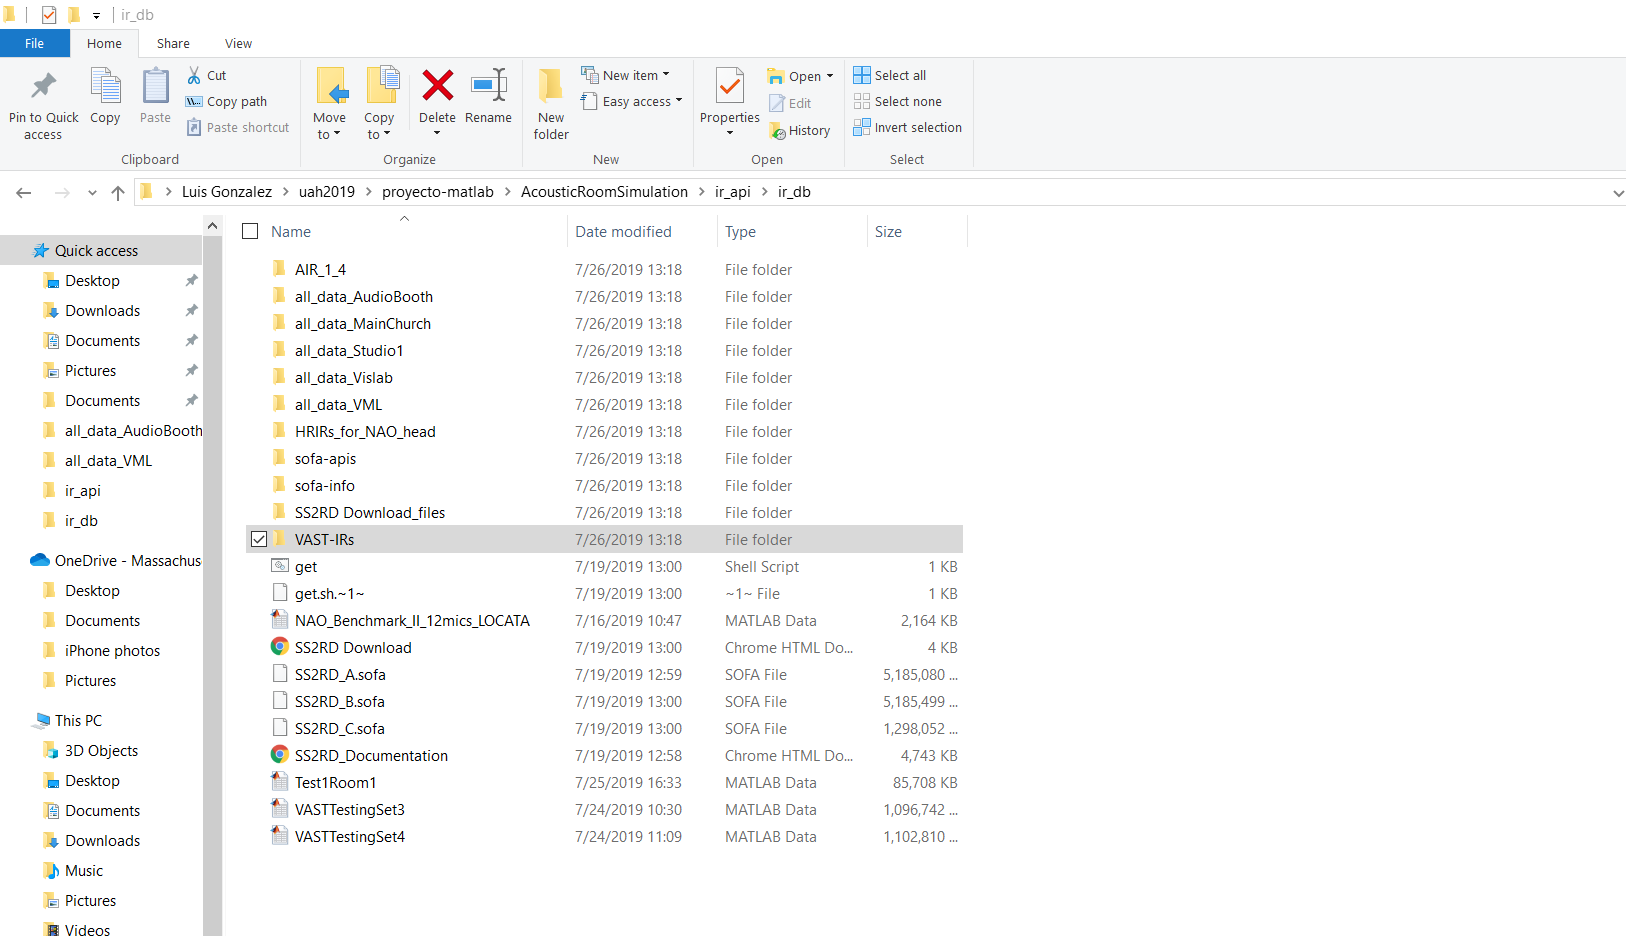
\includegraphics[width=0.9\textwidth]{filegestion.png}


Links to databases
\begin{itemize}
    \item LOCATA HRIRs \url{https://robot-ears.eu/measured-hrirs-for-prototype-head}
    \item NAO Steering vectors \url{http://www.ee.bgu.ac.il/~acl/register.php}
    \item VAST MITKemar Dataset \url{http://thevastproject.inria.fr/dataset/the-vast_mitkemar-dataset}
    \item Aachen Impulse Response Database \url{http://www.iks.rwth-aachen.de/en/research/tools-downloads/databases/aachen-impulse-response-database}
    \item S3A datasets \url{http://www.s3a-spatialaudio.org/datasets}
    \item POSZ Room Impulse Response \url{https://cvssp.org/soundzone/resource/Studio2RIR/index.html}
\end{itemize}

\end{document}
